\section{Statistical Learning}
% ======================================================================

\begin{sectionbox}
	\subsection{Definition}
	\textbf{Statistical Model}
	\begin{tablebox}{lll}
		Statistical Model: & $\{\mathbb X, \mathbb F, \P_θ ; θ \in \Theta\}$  \\
		Sample Space: & $Ω$\\
		Observation Space: & $\mathbb X$\\
		Sigma Algebra: & $\mathbb F$ \\
		Probability: & $\P_{\theta}$\\
		Test (decision rule): & $T:\mathbb X \mapsto \{\theta_{0},\theta_{1}\}, x \mapsto T(x)$\\
		Null Hypothesis: & $H_0: \theta \in \Theta_0 $  \\ 
		Alternative Hypothesis: &  $H_1: \theta \in \Theta_1 $\\
	\end{tablebox}
	\textbf{Cost Criterion $G_T$}:\\
	$G_T : \{\theta_0,\theta_1\} \mapsto [0,1], \theta \mapsto P(\{T(X)=1\};\theta)\\=E[T(X);\theta] = \int\limits_{\mathbb{X}}^{}{T(x)f_{X}(x;\theta)\diff x}$\\
	\textbf{Error Level $\alpha$}: $G_T(\theta_0) \leq \alpha$\\
	\textbf{Two Error Types}:\\
	False Alarm: $\theta = \theta_0, T(x)=1\\
	G_T(\theta_0)=P(\{T(X)=1\};\theta_0)$\\
	Detection Error: $\theta = \theta_1, T(x)=0\\
	1-G_T(\theta_1)=P(\{T(X)=0\};\theta_1)$\\
	
\end{sectionbox}

 
\begin{sectionbox}
	\subsection{Maximum Likelihood Test}
	\textbf{ML Ratio Test Statistic (Likelihood Ratio)}:\\	
	$R(x) = \begin{cases}
		\frac{f_{\X}(x;θ_1)}{f_{\X}(x;θ_0)}&;\quad f_X(x;\theta_0)>0\\
		\quad\quad\infty&;\quad f_X(x;\theta_0)=0$ and $f_X(x;\theta_1)>0
	\end{cases}$\\
	\textbf{ML Test}:\\	
	$T_{\ir ML} : \mathbb{X} \mapsto \{0,1\}, x\mapsto \begin{cases}
		1&;\quad R(X)>c\\
		0&;\quad$ otherwise
	$\end{cases}$\\
	if $c \ne 1$ False Alarm Error Probability can be adjusted $\rightarrow$ Neyman Pearson Test
\end{sectionbox}

\begin{sectionbox}
	\subsection{Neyman-Pearson-Test}
	The best test of $\P_0$ against $\P_1$\\
	NP-Test to the error level $\alpha$:\\
	%$x_{\alpha}$ is chosen as: $x_{\alpha} = (1-\alpha)$-quantile of $f_x(x;\theta_0)$\\
	If $P(\{R(x)=c;\theta_0\}) = f_{\X}(x_{\alpha}; θ_0)=0$:\\
	\parbox{15em}{$T_{\ir NP}(x) = \begin{cases} 1 & R(x) > c\\ 0 & R(x) < c \end{cases}$}
	\quad\quad \parbox{15em}{ Likelihood-Ratio: \\ $R(x) = \frac{f_{\X}(x; θ_1)}{f_{\X}(x; θ_0)}$ }\\
	If $P(\{R(x)=c;\theta_0\}) = f_{\X}(x_{\alpha}; θ_0)>0$:\\
	\parbox{15em}{$T_{\ir NP}(x) = \begin{cases} 1 & R(x) > c\\ γ & R(x) = c \\ 0 & R(x) < c \end{cases}$,}\\ 
	with $γ = \frac{α - P(\{R(x)>c;\theta_0\})}{P(\{R(x)=c;\theta_0\})}$ \quad error level $α$\\
	%Steps: For $α$ calculate $x_{α}$, then $c = R(x_{α})$\\
	\\
	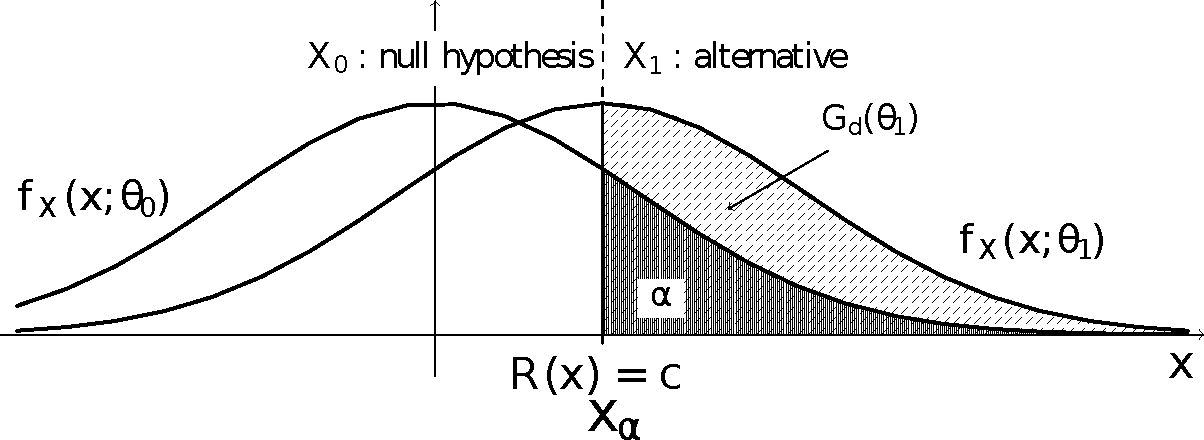
\includegraphics[width = \columnwidth]{tests}
	
	\textbf{Maximum Likelihood Detector:} \quad
	$T_{\ir ML}(x) = \begin{cases} 1 & R(x) > 1 \\ 0 & \text{otherwise} \end{cases}$\\
	\textbf{ROC Graphs:} plot $G_T(θ_1)$ as a function of $G_T(θ_0)$
\end{sectionbox}

\begin{sectionbox}
	\subsection{Bayes Test (MAP Test)}
	Prior knowledge about possible hypotheses:\\$\P(\{θ ∈ Θ_0 \}) + \P(\{θ ∈ Θ_1\}) =  1 $\\ 
	$T_{\ir Bayes} = \underset{T}{\operatorname{argmin}}\{P_{\epsilon}\}= 
	\begin{cases} 1 &;\quad\!\frac{f_{X}(x|θ_1)}{f_{X}(x|θ_0)} > c\\
	0&;\quad\text{otherwise}\end{cases} \\= \begin{cases} 1&;\quad \P(θ_1|x) > \P(θ_0|x) \\ 0 &;\quad \text{otherwise} \end{cases}\\
	\text{with}:\\ 
	P_{\epsilon} = P(\theta_0)G_T(\theta_0)+P(\theta_1)(1-G_T(\theta_1)),\quad c = \frac{P(\theta_0)}{P(\theta_1)}$\\\\
	\textbf{if} $P(\theta_0) = P(\theta_1) \implies T_{\ir Bayes} = T_{\ir ML}$\\\\
	\textbf{Multiple Hypothesis} $\{\theta_0,...,\theta_k\}; \mathbb{X}_0,...,\mathbb{X}_k \in \mathbb{X}$:\\
	$T_{\ir Bayes} = \underset{k\in1,...,K}{\operatorname{argmin}}\{P(\theta_k|x)\}$\\\\
	\textbf{Loss Function}:\\
	$L(T(x), θ) = \begin{cases} L_0 &;\quad T(x) = 1, \text{ but }θ = θ_0\quad \text{(FALSE ALARM)} \\
	L_1 &;\quad T(x) = 0, \text{ but }θ = θ_1\quad \text{(DETEC. ERROR)}\\
	0 &;\quad \text{otherwise} \end{cases}$\\
	$L_i$ denotes the Loss Value in cases where the correct decision parameter $θ_i$ is missed.\\
	$\operatorname{Risk}(T) = \E[L(T(\X), θ)] = \E [\E [L(T(x), θ)|x = \X ]]$\\
\end{sectionbox}

\begin{sectionbox}
	\subsection{Linear Alternative Tests}
	
	Estimate normal vector $\vec w^\top$ and $w_0$, which separate $\mathbb X$ into $\mathbb X_0$ and $\mathbb X_1$\\
	$\log R(\vec x) = -\frac{1}{2}\ln(\frac{\det(\ma C_1)}{\det(\ma C_0)}) - \frac{1}{2}(\vec x- \vec{μ}_1)^\top\ma C_1^{-1}(\vec x- \vec{μ}_1) +\\+\frac{1}{2}(\vec x- \vec{μ}_0)^\top\ma C_0^{-1}(\vec x- \vec{μ}_0) = \ln(\frac{P(\theta\in\Theta_0)}{P(\theta\in\Theta_1)})$ (seperating surface)\\\\
	For Gaussian $f_X(x; \mu_k, C_k)$ with $θ_0$ and $θ_1$ corresponding to $\{\mu_0,C_0\}$ and $\{\mu_1, C_1\}$, it follows that
	\begin{itemize}
		\item if $C_0 \ne C_1$, $logR(x) = 0$ is non-linear and the separating surfaces are surfaces of second order:
		parabolic, hyperbolic, or elliptic surfaces.
		\item if $C_0 = C_1$, $logR(x) = 0$ is affine and thus defines a hyperplane in $\mathbb{X}$ which decomposes $\mathbb{X}$ into $\mathbb{X}_0$ and $\mathbb{X}_1$, i.e.,\\
		$T: \mathbb X \ra \R, \vec x \mapsto \begin{cases} 1 & \vec w^\top \vec x > w_0\\ 0 & \text{otherwise}\end{cases}$\\
		\begin{itemize}
			\item case 1: $\ma C_0 = \ma C_1 = \sigma^2\ma I_N$\\
			$\vec w^\top = (\vec\mu_1-\vec\mu_0)^\top,\\
			w_0= \frac{1}{2}(\vec\mu_1^\top\vec\mu_1-\vec\mu_0^\top\vec\mu_0) -\sigma^2\ln(\frac{P(\theta\in\Theta_1)}{P(\theta\in\Theta_0)})$\\
			$\vec w$ colinear with $(\vec \mu_1-\vec \mu_0)\\\implies \text{hyperplane orthogonal to } (\vec \mu_1-\vec \mu_0)$ 
			\item case 2: $\ma C_0 = \ma C_1 = \ma C$\\
			$\vec w^\top = (\vec\mu_1-\vec\mu_0)^\top\ma C^{-1},\\
			w_0= \frac{1}{2}(\vec {μ}_1 - \vec{μ}_0)^\top \ma C^{-1} (\vec {μ}_1 + \vec{μ}_0) -	\ln(\frac{P(\theta\in\Theta_1)}{P(\theta\in\Theta_0)})$\\
			in general $\vec w$ \textbf{not} colinear with $(\vec \mu_1-\vec \mu_0)\\\implies \text{hyperplane \textbf{not} orthogonal to } (\vec \mu_1-\vec \mu_0)$ 
		\end{itemize}
		\item if $C_0 = C_1$ and $\mu_0 = −\mu_1$, $log R(x) = 0$ is linear and defines a separating hyperplane in $\mathbb{X}$ which contains the origin, i.e.,\\
		$T: \mathbb X \ra \R, \vec x \mapsto \begin{cases} 1 & \vec w^\top \vec x > 0\\ 0 & \text{otherwise}\end{cases}$\\
	\end{itemize}
	
	
	% Bild aus Part7 p 197!!!
	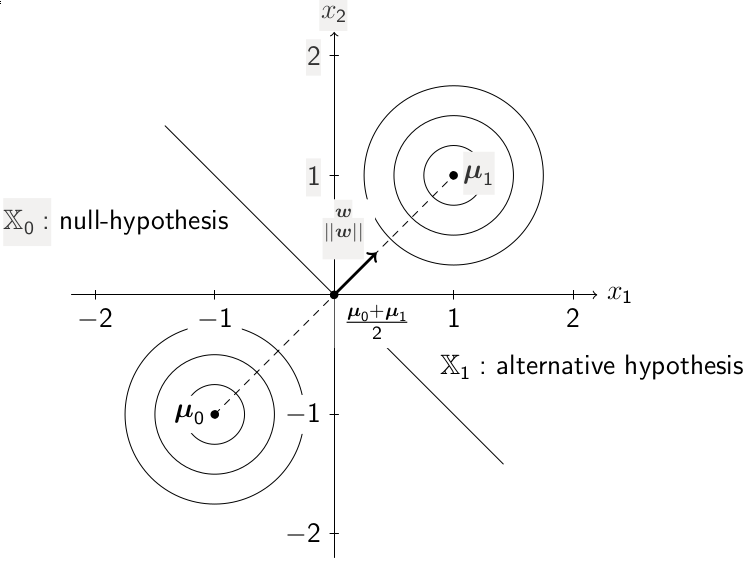
\includegraphics[width = \columnwidth]{linest2}
	
\end{sectionbox}